\section{Other Features}
\subsection{Collision detectors}
\red{JS}
\subsection{Integration methods}
\red{Karen}
\subsection{Lazy evaluation and automatic updating}
\label{sec:lazy}
Most kinematics libraries have a strict workflow that must be followed in order to produce correct results in a timely manner. Typically this workflow requires that all joint positions must be set and then all transforms must be computed before the transformation of a specific frame may be queried. This is a wasteful and inefficient approach for many applications.

For example, a dexterous robot manipulator may have seven links from the base to the end effector, but then it may have three fingers which each have three links. While iteratively performing inverse kinematics, it will be necessary to repeatedly compute the seven matrix transformations that go from the base to the end effector, but the transforms of the nine finger links are unnecessary. A naive approach to updating kinematics will compute all 16 transforms, even though only 7 are necessary. This means that over 56\% of the computational effort of the forward kinematics is wasted. When iteratively solving an inverse kinematics problem, the bulk of time is spent computing forward kinematics. This means that intelligently updating the forward kinematics could yield a nearly 50\% reduction in computation time for this example. Similar (and more extreme) examples could be imagined for robots with multiple limbs.

Strict workflow requirements can also lead to bugs in code. If a human programmer is not familiar with the correct workflow, does not fully understand the necessary order of operations, or simply makes a programming error, then there may be bugs in a complex controller which would produce incorrect results. Incorrect results on a dexterous manipulator could cause a task to fail and damage the robot. Incorrect results on a high-powered robot could severely damage the robot and even endanger human lives.

\subsubsection{Design}

KIDO resolves those concerns using lazy evaluation and automatic updating. Most kinematic and dynamic quantities in KIDO are automatically updated and lazily evaluated (see section \ref{sec:lazy_exception} for the exceptions). \textit{Automatic updating} means that you never need to explicitly call any kind of ``update'' function in order to get the correct output based on your most recent input. \textit{Lazy evaluation} means that expensive computations are held off until they are absolutely required by the user. Combined, these two add a decisive level of code safety to applications that use KIDO, and they cut out a considerable degree of potential waste, both while making the library easier to use. This is accomplished with the following setup:

\begin{itemize}
  \item Mutator and accessor methods (a.k.a. setters and getters) intercept all interactions with the internal states and properties of kinematic objects.
  \item Dirty flags are used to keep track of which quantities are out of date, and the dirtiness gets propagated to all dependencies.
  \item Accessor methods will check any relevant dirty flags and perform computations as necessary.
  \item Mutator methods will trigger dirty flags.
\end{itemize}

A visual example of this scheme applied to forward kinematics can be seen in figure \ref{fig:lazy}. Note that the propagation of dirty flags throughout the kinematic structure will short-circuit any time a kinematic object already knows that it is dirty. This prevents the bookkeeping from having $O(N^2)$ complexity when all $N$ joints in the kinematic structure undergo changes.

To facilitate this lazy evaluation, KIDO abides by logical const-correctness (rather than physical const-correctness). The values that are lazily evaluated are stored as mutable members of their class, allowing the \texttt{getX()} functions to be const member functions. However, because of this mutability, the const-qualifier on member functions does \textbf{not} guarantee thread-safety. Currently, the only guaranteed way to ensure thread-safety with KIDO is to spawn identical copies of the kinematic structures for each thread. This is done easily with the various \texttt{clone()} functions throughout KIDO. To spawn an identical copy of a single Skeleton, simply call \texttt{Skeleton::clone()} on it. To spawn an identical copy of a whole environment, you can use the \texttt{simulation::World::clone()} function.

\begin{figure}
  \centering
  \subfigure[][\label{fig:lazy_1}Everything is cached]{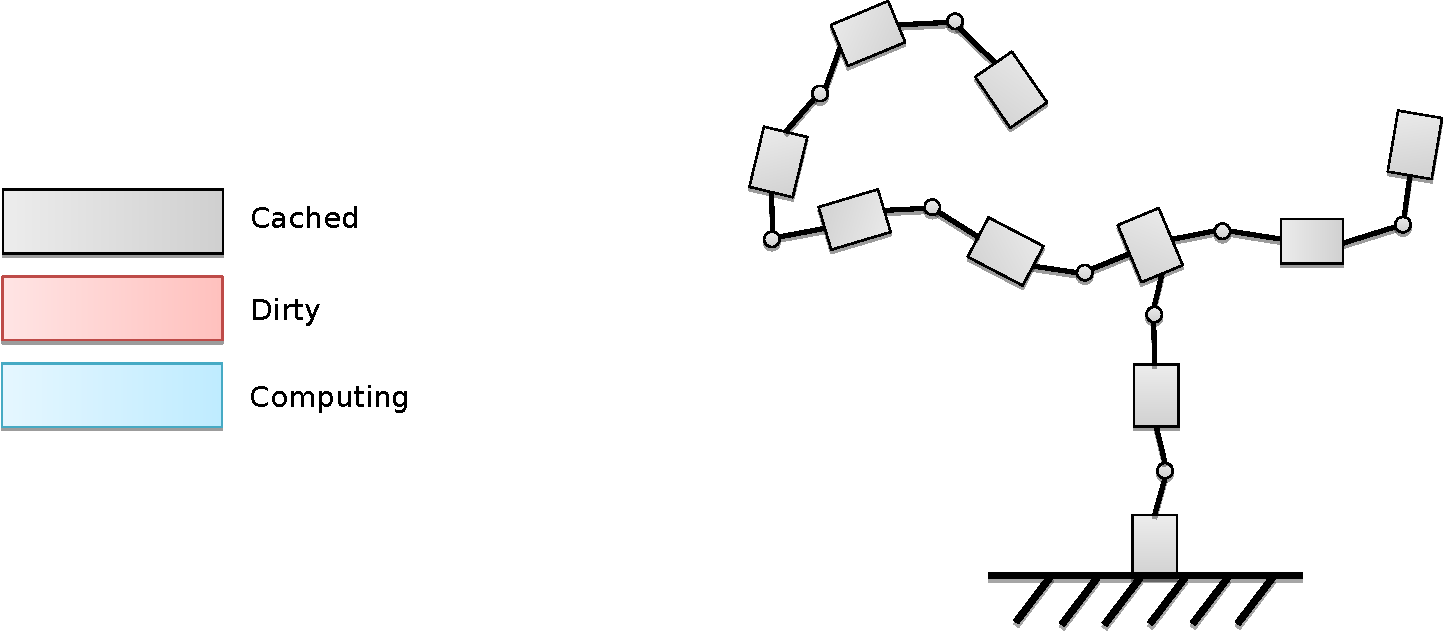
\includegraphics[width=0.98\textwidth]{fig/lazy_1.pdf}}
  
  \subfigure[][\label{fig:lazy_2}Some joint values have changed]{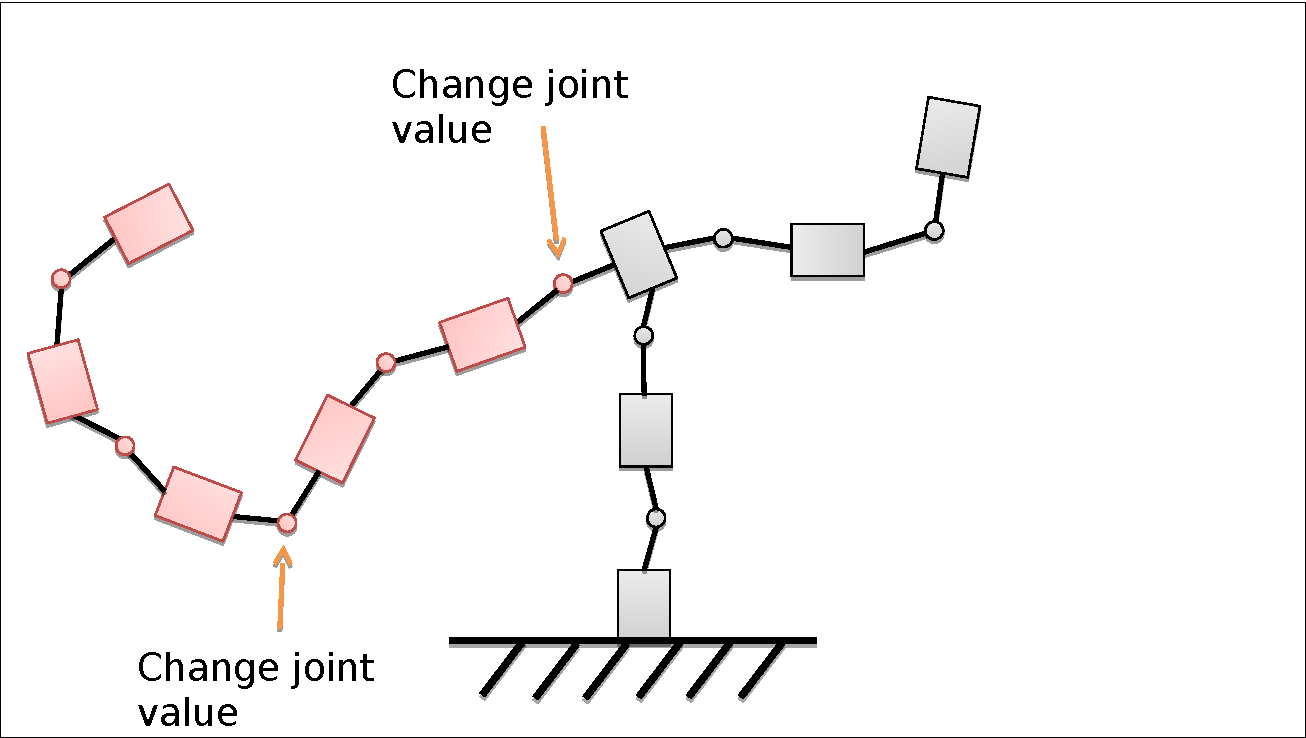
\includegraphics[width=0.44\textwidth]{fig/lazy_2.pdf}}
  \subfigure[][\label{fig:lazy_3}A dirty transform is queried]{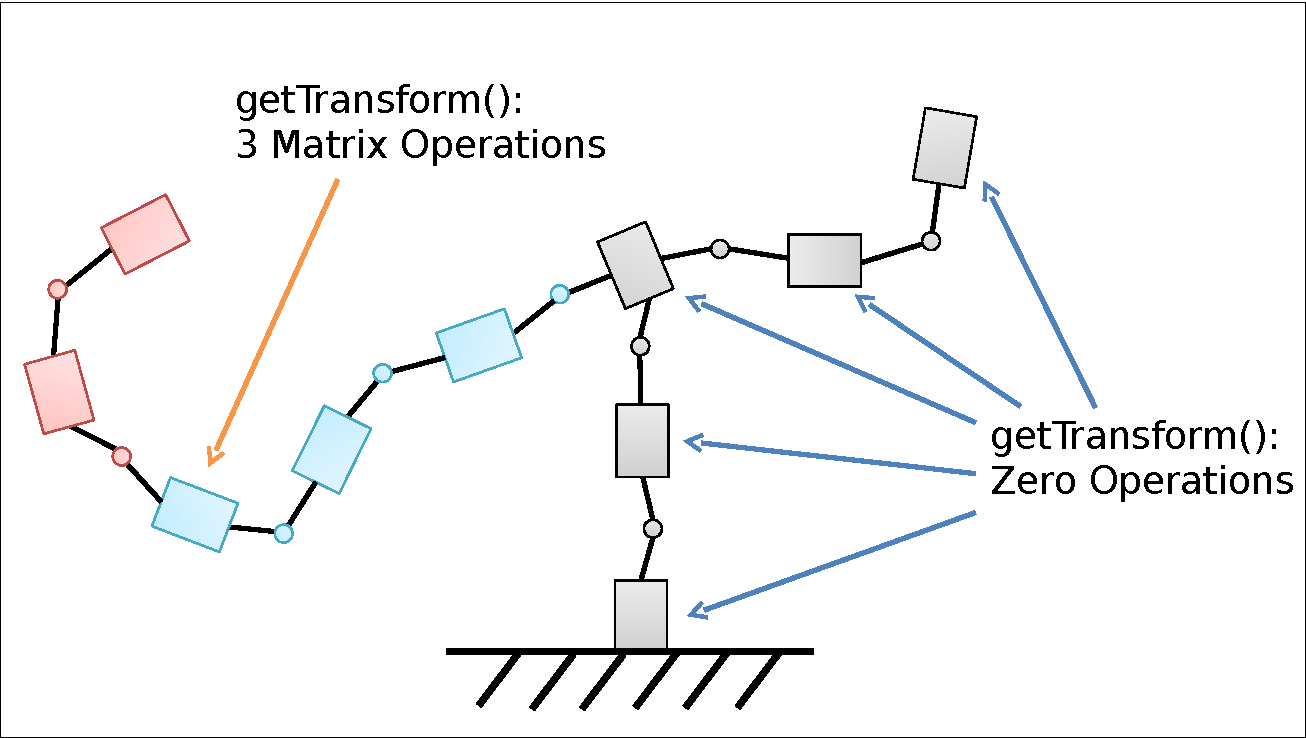
\includegraphics[width=0.44\textwidth]{fig/lazy_3.pdf}}
  
  \subfigure[][\label{fig:lazy_4}Cached transforms can be used freely]{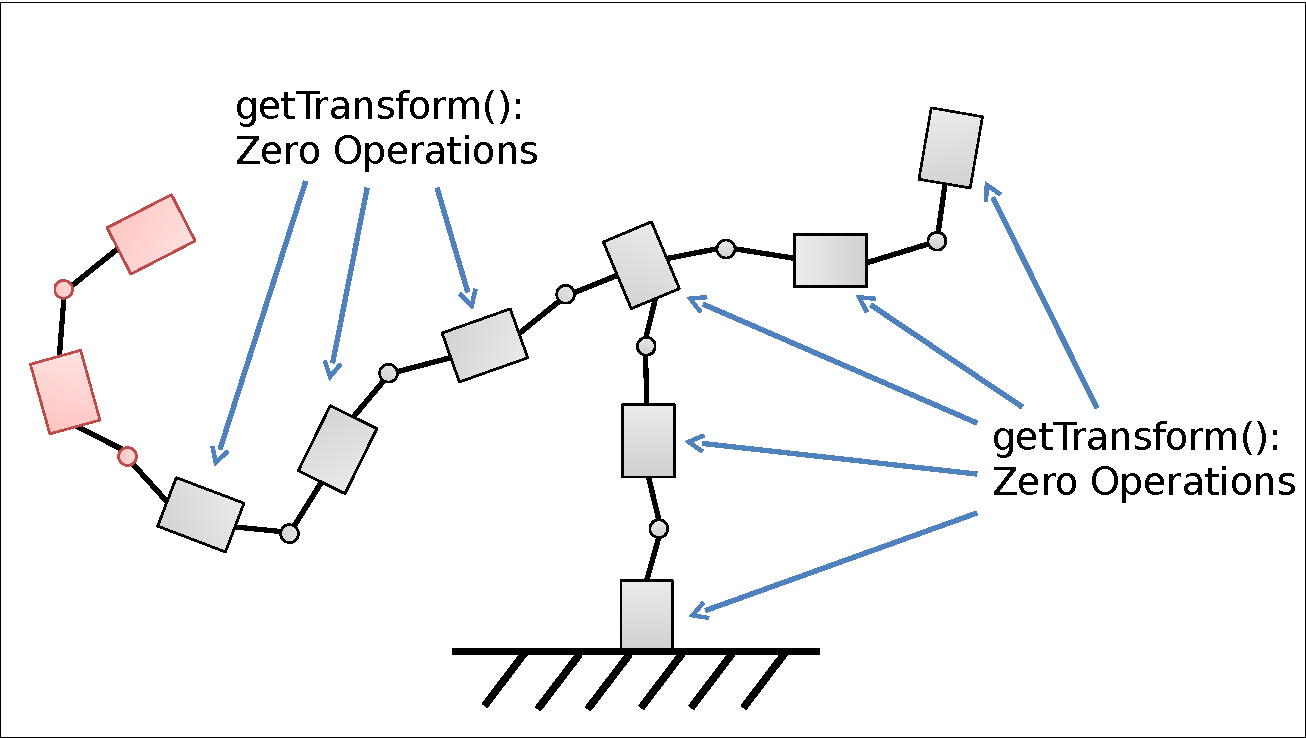
\includegraphics[width=0.44\textwidth]{fig/lazy_4.pdf}}
  \subfigure[][\label{fig:lazy_5}Another dirty transform is queried]{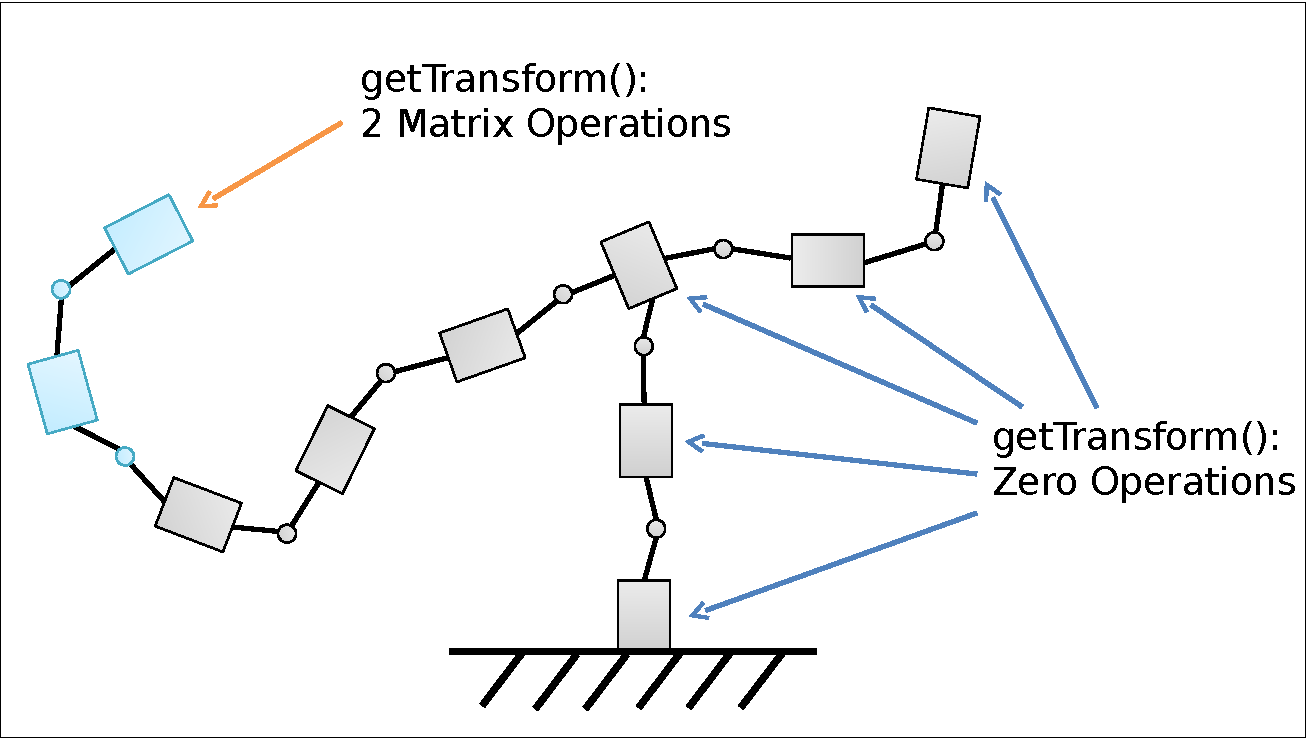
\includegraphics[width=0.44\textwidth]{fig/lazy_5.pdf}}
  \caption{Illustration of lazy evaluation for forward kinematics}
  \label{fig:lazy}
\end{figure}

In some cases, it might be undesirable to delay the computations until the time that they are requested. For example, if a real-time controller has strict scheduling requirements, there might be a specific time window which is best suited for performing heavy computations. In that case, KIDO provides a \texttt{Skeleton::computeForwardKinematics()} function which will compute all the forward kinematics within a Skeleton instead of waiting for it to be automatically updated. There are also \texttt{Skeleton::computeForwardDynamics()} and \texttt{Skeleton::computeInverseDynamics()} functions which will compute all the various dynamics parameters instead of waiting to evaluate them as needed.

\subsubsection{Exceptions: Forward and Inverse Dynamics Updating}
\label{sec:lazy_exception}
Even though forward kinematics is updated automatically, neither forward nor inverse dynamics have this quality. Individual dynamics parameters---such as the mass matrix, Coriolis forces, and articulated inertia---are updated automatically, but KIDO will \textbf{not} automatically compute the body accelerations due to the current joint torques or vice versa. This is due to the ambiguous nature of how the user might want to utilize the library: Do they want to simulate forward to see a result or compute the inverse dynamics to inform a controller? In order to compute one or the other automatically, the library would need to make an assumption about which one the user is interested in, but KIDO is meant to be suitable for both. Instead, KIDO requires the user to specifically request one or the other each time they want the results:

\begin{itemize}
  \item \textbf{\texttt{Skeleton::computeForwardDynamics()}} should be used to compute the accelerations of all the BodyNodes given the current generalized forces (or more generally, the current commands) of their joints.
  \item \textbf{\texttt{Skeleton::computeInverseDynamics()}} should be used to compute the generalized forces needed by the joints in order to achieve the current accelerations of the BodyNodes.
\end{itemize}

The results of each call will show up in the joint states of the Skeleton. The results of \texttt{computeForwardDynamics()} will show up in \texttt{Joint::getAccelerations()} and then by extension \texttt{BodyNode::getSpatialAcceleration()}, \texttt{getLinearAcceleration()}, and \texttt{getAngularAcceleration()}. The results of \texttt{computeInverseDynamics()} will show up in \texttt{Joint::getForces()} and by extension \texttt{Skeleton::getForces()}.

In both cases, the functions make use of kinematics and dynamics parameters which are cached and lazily evaluated, so making redundant calls to these functions is not prohibitively expensive, although it is still not completely free of charge.

\subsection{Extensible data structures}

There are countless applications for kinematics and dynamics software, and the developers of KIDO do not anticipate that we could possibly account for all use cases. Instead of limiting the potential applications of the library with a closed-off design, we have made the kinematics and dynamics structures extensible by introducing the concepts of \textbf{Addon}s and \textbf{Node}s.

\textbf{Addon}s and \textbf{Node}s have some practical and semantic differences, but their overarching motivation is the same: They provide a way to embed arbitrary data and functionality into kinematic and dynamic structures. For example, if you want to have a custom sensor type that can be attached to a body on your robot, you could create a custom \textbf{Node} and attach instances of your \textit{SensorNode} on whichever bodies need it.

Any concept can be encapsulated into either an \textbf{Addon} or a \textbf{Node} as long as its contents can be decomposed into a \textbf{State} structure and/or a \textbf{Properties} structure (or neither if the concept contains no information at all). To fully understand whether an Addon or a Node should be used for your purposes, the following subsections will explain the difference, but the differences can be boiled down to these:

\begin{itemize}
  \item A \textbf{BodyNode} can only contain a single instance of any particular type of \textbf{Addon}, but it can contain arbitrarily many of any particular type of \textbf{Node}.
  \item \textbf{Node}s can only be attached to \textbf{BodyNode}s, but \textbf{Addon}s can be attached to any class that inherits \textbf{AddonManager} (e.g. \textbf{Joint}, \textbf{Skeleton}, \textbf{EndEffector}).
\end{itemize}

\subsubsection{Addons}
\label{sec:addons}

There may be times where you have developed a novel algorithm that requires extra contextual information that might not be natively available in KIDO. For example, you might have computed an occupancy grid for some geometry, but KIDO does not natively support occupancy grids. Nevertheless, you want the information to be embedded in the geometric object; you want it to be saved as part of the object's \textbf{Properties}, and you want it to get copied over whenever the object is cloned.

You could achieve this by defining an \textit{OccupancyGrid} class that inherits the \textbf{Addon} class. Then you could embed an instance of an \textit{OccupancyGrid} class into the \textbf{ShapeNode} instance that holds the geometric data for which the occupancy grid was calculated:

\begin{lstlisting}
shapeNode->create<OccupancyGrid>(gridInfo);
\end{lstlisting}

You can then retrieve it with:

\begin{lstlisting}
OccupancyGrid* grid = shapeNode->get<OccupancyGrid>();
\end{lstlisting}

If the object named \texttt{shapeNode} has never created or been given an \texttt{OccupancyGrid} object, this function will return a \texttt{nullptr} by default. It is always a good idea to check whether the \textbf{Addon} pointer that gets returned is a \texttt{nullptr}, because KIDO does not throw any exceptions or assertions when you request an \textbf{Addon} that is not present in the object.

There are many native Addons in KIDO:

\begin{itemize}
  \item \textbf{Support} which is an Addon for \textbf{EndEffector}
  \item \textbf{RevoluteJoint::Addon} which contains unique properties for \textbf{RevoluteJoint}
  \item \textbf{PrismaticJoint::Addon} which contains unique properties for \textbf{PrismaticJoint}
  \item (All the other six Joint-type Addons)
  \item \todo[MXG]{Mention the Addons for ShapeFrame once they are finished}
\end{itemize}

In some cases, such as the Joint-type Addons, the Addon is crucial for the object to function correctly. In other cases, such as the \textbf{Support} class, the Addon simply provides extra features. It might seem counter-intuitive to put critical property information into an Addon if the class cannot function without it, but there is a strong motivation for this: When the \textbf{Skeleton::ExtendedProperties} is retrieved, it pulls in all the \textbf{Properties} of all the \textbf{BodyNode}s, \textbf{Node}s, and \textbf{Joint}s in the \textbf{Skeleton}, as well as the \textbf{Properties} of all the \textbf{Addon}s attached to those \textbf{BodyNode}s, \textbf{Node}s, and \textbf{Joint}s. This means that there is no special handling required in order to save all the unique property information for each different Joint-type; all their unique properties are stored in \textbf{Addon}s, and the Properties of those \textbf{Addon}s will get sucked into the \textbf{Skeleton::ExtendedProperties} automatically.

By creating your own custom Addons and attaching them to objects in Skeletons, you can extend the scope of a Skeleton's \textbf{State} and \textbf{ExtendedProperties}. The State of your Addon will be embedded into the \textbf{Skeleton::State}, and the Properties of your Addon will be embedded into the \textbf{Skeleton::ExtendedProperties}. Creating your own custom Addon involves---at a minimum---inheriting the class \textbf{kido::common::Addon} and then overriding the \textbf{Addon::cloneAddon} function. Additionally, if your Addon has a \textbf{State}, then you should also override the functions \textbf{Addon::setAddonState(const State\&)} and \textbf{Addon::getAddonState()}. Neglecting to override those functions will cause \textbf{Skeleton::State} to treat your Addon as though it has no State. Similarly, if your Addon has \textbf{Properties}, then you should override the functions \textbf{Addon::setAddonProperties(const Properties\&)} and \textbf{Addon::getAddonProperties()}. Neglecting to override these will cause \textbf{Skeleton::ExtendedProperties} to treat your Addon as though it has no Properties. Also note that the constructor of your Addon is expected to take an \textbf{AddonManager*} as its first argument; it can have any number of arbitrary argument types after that.

The most common use case of an Addon is to embed plain old data (POD) into the Properties or State of a Skeleton. To accommodate this, we offer two templated classes which take care of constructing an Addon with \textbf{State} and/or \textbf{Properties} that can live happily within a Skeleton:

\begin{itemize}
  \item \textbf{AddonWithProtectedPropertiesInSkeleton} is suitable for Addons which only has a POD \textbf{Properties} and no \textbf{State}.
  \item \textbf{AddonWithProtectedStateAndPropertiesInSkeleton} is suitable for Addons which have both a POD \textbf{State} and a POD \textbf{Properties}.
\end{itemize}

The template arguments of these classes work as follows:

\begin{itemize}
  \item The class type that inherits this class. These are CRTP classes.
  \item (Only for AddonWithProtectedStateAndPropertiesInSkeleton) The POD \textbf{State} type
  \item The POD \textbf{Properties} type
  \item The type of AddonManager that this class is intended for. Pass in \texttt{AddonManager} if the type of AddonManager is irrelevant.
  \item (Only for AddonWithProtectedStateAndPropertiesInSkeleton) The function that should be called whenever the State of the Addon is updated.
  \item The function that should be called whenever the Properties of the Addon are updated
\end{itemize}

The update functions that are used for the final template argument(s) must accept a single argument, which will be a pointer to the full Addon class. CRTP (Curiously Recurring Template Pattern) is used to make this possible.

The \textbf{State} and \textbf{Properties} are protected for this type of Addon to ensure that all changes to the \textbf{Properties} are registered by the \textbf{Skeleton}. Otherwise, \textbf{Skeleton}s would not be able to correctly keep track of their ``version'' number \todo[MXG]{We should probably have a section about Skeleton version and cite it here}. This can be inconvenient if the POD \textbf{State} or \textbf{Properties} structures have many fields that need to be accessed or changed, because then accessor and mutator functions are needed for each one. This can entail a troublesome amount of typing, and worse yet: When writing mutator functions, you must be sure to call the correct update functions, and increment the Skeleton's version number if a property is being changed.

To avoid the hassle and dangers of writing many accessor and mutator functions, KIDO provides a few macros which can take of this:

\paragraph{KIDO\_DYNAMICS\_SET\_GET\_ADDON\_PROPERTY} will create a setter and getter function for a variable in the Properties POD. The first argument for this macro is the variable type, and the second argument is the variable name. There is also:
\begin{itemize}
  \item \textbf{KIDO\_DYNAMICS\_SET\_ADDON\_PROPERTY} which will only create the set
  \item \textbf{KIDO\_DYNAMICS\_GET\_ADDON\_PROPERTY} which will only create the get
\end{itemize} 

\paragraph{KIDO\_DYNAMICS\_SET\_GET\_ADDON\_PROPERTY\_ARRAY} can be used to access and mutate the individual components of an array or vector field within the POD \textbf{Properties} structure. For variable names whose plural form is ``irregular'' (i.e. is not the same as adding `s' to the end), there is also 

\begin{itemize}
  \item \textbf{KIDO\_DYNAMICS\_IRREGULAR\_SET\_GET\_ADDON\_PROPERTY\_ARRAY} which allows you to specify the singular and plural forms of the name.
\end{itemize}

There are more macros, similar to these, which address a variety of use cases. Although C-macros can be strange and clumsy, they can save a significant amount of typing and prevent errors that may result from forgetfulness.

\subsubsection{Nodes}
\label{sec:nodes}

\textbf{Node}s are conceptually similar to \textbf{Addon}s, so this section will focus on what makes \textbf{Node}s different from \textbf{Addon}s. Reading the previous section (\ref{sec:addons}) on \textbf{Addon}s before this section is recommended.

Only one instance of any particular type of \textbf{Addon} can be embedded into a single AddonManager. \textbf{Node}s differ from this in that any number of a \textbf{Node} type can be attached to a \textbf{BodyNode}. This brings up another difference: A \textbf{Node} can only be attached to a \textbf{BodyNode}, whereas an \textbf{Addon} can be attached to anything that inherits the AddonManager class. Each \textbf{Node} also requires a name, which is not necessary for an \textbf{Addon}. Moreover, each \textbf{Node} of any given \textbf{Node} type within a \textbf{Skeleton} must have a unique name. \textbf{Node}s can be accessed by name and type through their \textbf{Skeleton}, for example:

\begin{lstlisting}
// Assume skeleton is a SkeletonPtr type:
EndEffector* hand = skeleton->getNode<EndEffector>("left_hand");
\end{lstlisting}

Even though \textbf{Node}s are accessible through the \textbf{Skeleton}, they are not owned by the Skeleton; they are owned by the \textbf{BodyNode} to which they are attached. If the \textbf{BodyNode} is moved to a new \textbf{Skeleton}, all \textbf{Node}s that are attached to it will follow. However, the indexing of the \textbf{Node}s may change after being moved into a new Skeleton, and the names of the \textbf{Node}s may change (by appending a number to the string) if there is a name collision with any \textbf{Node}s of the same type that were already in the \textbf{Skeleton}. If a name change occurs, a message will be printed to \texttt{stdout}, and a \textbf{NameChangedSignal} will emanate from the \textbf{Node} whose name needed to be changed. When a whole \textbf{Skeleton} is cloned into a new \textbf{Skeleton}, the names of its \textbf{Node}s are guaranteed to remain the same, and the indexing of the \textbf{Node}s is guaranteed to remain the same.

The defining feature of a \textbf{Node} is that it is something which belongs to a \textbf{BodyNode} in some sense. \textbf{BodyNode} is a special case of the \textbf{Node} class; it is a \textbf{Node} which belongs to itself. Because of this, it has its own specialized management semantics (described in section \ref{sec:skeleton_modeling}). Most other \textbf{Node} types will simply inherit the \textbf{AccessoryNode} class which allows them to be detached from their \textbf{BodyNode} by calling the \textbf{remove()} function on them. When a \textbf{Node} is removed from its \textbf{BodyNode}, it can no longer be accessed by calling any \textbf{getNode} function from the \textbf{BodyNode} or \textbf{Skeleton} that it had been attached to. If no strong references (such a \textbf{NodePtr}) remain for a removed \textbf{Node}, then the \textbf{Node} instance will be deleted. If a strong reference does exist, then the \textbf{Node} will continue to function as normal, except any features which would normally access it through a \textbf{getNode} call will no longer work. The Node will also have \textbf{INVALID\_INDEX} as its index within the \textbf{BodyNode} and within the \textbf{Skeleton} (note that this does not mean you can access the Node using \textbf{INVALID\_INDEX}). A removed \textbf{AccessoryNode} can be reattached---if and only if a strong reference to it remains---by calling the \textbf{reattach()} function on it.

When creating a custom \textbf{Node} type, you will most likely want to inherit \textbf{AccessoryNode}, because it will provide the interface for removing and reattaching that was described in the previous paragraph. If your \textbf{Node} inherits the \textbf{Frame} class in some way, you might also want to have it inherit the \textbf{TemplatedJacobianNode} class in order to provide it with an interface for computing Jacobians. Note that the Node class does not allow multiple-inheritance (just like the Addon class), so if you have an implementation of some features which you would like to share among a number of different \textbf{Node} types, we advise you to use CRTP-style mix-in classes, like the \textbf{AccessoryNode} class.

Just like the \textbf{Addon} class, the \textbf{Node} class has a concept of \textbf{State}, \textbf{Properties}, and cloning. It also has a concept of naming. The following functions \textbf{need} to be overridden by inheriting classes:

\begin{lstlisting}
// Create a new Node which is identical to this one, except it will be attached to
// the BodyNode named bn.
Node* cloneNode(BodyNode* bn) const;

// Change the name of this Node. When implementing this function, you must be sure
// to call the protected function Node::registerNameChange(const std::string&),
// otherwise the Skeleton would be left unaware of the name change. Note that if
// the new name collides with an already existing name, then
// Node::registerNameChange(~) will let you know this by returning the modified
// version of the name. Otherwise, it will send back the name that you passed in.
//
// You should return the final name, as given back by Node::registerNameChange(~),
// to convey to the user what the final name will be.
const std::string& setName(const std::string& newName);

// Different Nodes might store their names in different ways, so this function is
// pure virtual in order to give the user the freedom to decide how their Node's
// name is stored.
const std::string& getName() const;
\end{lstlisting}

Additionally, if the Node has State data, the following functions should be overridden:

\begin{lstlisting}
// Set the State of the Node given a reference to a const Node::State object. You
// will be required to downcast the reference to the correct type for your Node.
// Even though KIDO guarantees that the incoming reference will always be
// appropriate type for your Node type, this guarantee does not apply to any time
// that a user decides to invoke this function. Therefore, a static_cast is
// recommended for downcasting if performance is the most important factor, but
// only a dynamic_cast can ensure that the function is safe from malicious or
// careless users.
void setNodeState(const Node::State& otherState);

// Return a pointer containing a newly instantiated version of the Node::State
// for your Node type.
std::unique_ptr<Node::State> getNodeState() const;
\end{lstlisting}

Similarly, if the Node has Properties data, the following functions should be overridden:

\begin{lstlisting}
// Similar to setNodeState (see above), except for Properties data
void setNodeProperties(const Node::Properties& otherProperties);

// Similar to getNodeState (see above), except for Properties data
std::unique_ptr<Node::Properties> getNodeProperties() const;
\end{lstlisting}

In some cases, the \textbf{State} or \textbf{Properties} of a particular \textbf{Node} type might contain a significant amount of data which would be slow or wasteful to frequently allocate and deallocate. For cases like this, the following functions will pass a \textbf{Node::State} or \textbf{Node::Properties} pointer which can be modified directly to match the current \textbf{State} or \textbf{Properties} of the Node. This avoids the need to allocate and deallocate the \textbf{State} or \textbf{Properties} from the heap:

\begin{lstlisting}
// You can copy the state information directly instead of allocating a copy in
// new memory.
void copyNodeStateTo(std::unique_ptr<Node::State>& outputState) const;

// You can copy the property information directly instead of allocating a copy in
// new memory.
void copyNodePropertiesTo(
    std::unique_ptr<Node::Properties>& outputProperties) const;
\end{lstlisting}

This is all that is needed to create a fully functional Node that is compatible with KIDO and can be attached to a BodyNode.

\subsection{History recorder}
\todo[MXG]{It doesn't look like we'll have this in time for the next major release, although it will probably be available for the next minor release. Will it be possible to update this tech report as we add features and make changes?}
\subsection{Optimization interface}
\label{sec:optimizer}
\red{Grey}
\subsection{Extensible GUI}
\red{JS}
